% Unit 118 terjemahan Bahasa Indonesia dari chapter8.tex baris 1850--1999.
% Sumber: Methods of Algebra, Volume 2, commit
% 9a5803ff77dd3257484cb177f851a73770a59dd3 (CC BY 4.0).
% stable-unit-id: o014.aljabr2.chapter8.mapping-cone-revisited
% Cakupan: Bagian 8.10 lengkap, hingga sebelum Latihan.
% Koreksi sumber terpaksa: baris 1855 f(x)->F(x); baris 1957 -f[-1]->-\phi[-1].

% segment-id: o014.li2.chapter8.mapping-cone-revisited.h001
\section{Meninjau kembali kerucut pemetaan}\label{sec:mapping-cone-revisited}
\hypertarget{o014.aljabr2.chapter8.mapping-cone-revisited}{ }
% segment-id: o014.li2.chapter8.mapping-cone-revisited.p001
Seperti telah terlihat dalam \S\ref{sec:mapping-cone} dan
\S\ref{sec:derived-cat}, kerucut pemetaan $\Cone(f)$ berperan penting
dalam teori kompleks dan kajian kategori turunan. Tujuan bagian ini ialah
menafsirkannya melalui korespondensi Dold--Kan dan menjelaskan mengapa
kerucut pemetaan memang sebuah ``kerucut''. Lebih tepatnya, yang akan
ditelaah ialah versi kompleks rantai dari kerucut pemetaan; lihat
Catatan~\ref{rem:cone-chain}.

% segment-id: o014.li2.chapter8.mapping-cone-revisited.p002
Kita mulai dengan kerucut dan silinder pemetaan dalam topologi. Tinjau
pemetaan kontinu $F:\mathcal{X}\to\mathcal{Y}$ dengan
$\mathcal{X}\neq\emptyset$. Silinder pemetaan yang bersesuaian ialah ruang
hasil bagi
% segment-id: o014.li2.chapter8.mapping-cone-revisited.q001
\begin{equation*}
	\Cyl_{\mathrm{top}}(F) := \dfrac{(\mathcal{X} \times [0, 1]) \sqcup \mathcal{Y}}{\forall x \in \mathcal{X}, \; (x, 1) \sim F(x)},
\end{equation*}
dengan $\times$ (atau $\sqcup$) menyatakan hasil kali (atau gabungan
terpisah) ruang topologis. Kerucut pemetaan didefinisikan oleh
% segment-id: o014.li2.chapter8.mapping-cone-revisited.q002
\begin{equation*}\begin{aligned}
	\Cone_{\mathrm{top}}(F) & := \dfrac{(\mathcal{X} \times [0, 1]) \sqcup \mathcal{Y}}{\forall x \in \mathcal{X}, \; (x, 1) \sim F(x), \; (x, 0) \sim (\star, 0)} \\
	& \simeq \dfrac{\Cyl_{\mathrm{top}}(F)}{\forall x \in \mathcal{X}, \; (x, 0) \sim (\star, 0)},
\end{aligned}\end{equation*}
di mana $\star\in\mathcal{X}$ titik sebarang. Secara intuitif,
$\mathcal{X}\times[0,1]$ dapat dibayangkan sebagai tabung dengan penampang
$\mathcal{X}$. Silinder $\Cyl_{\mathrm{top}}(F)$ diperoleh dengan
merekatkan ujung tabung $\mathcal{X}\times\{1\}$ pada $\mathcal{Y}$
melalui $F$, sedangkan $\Cone_{\mathrm{top}}(F)$ selanjutnya mengerutkan
ujung $\mathcal{X}\times\{0\}$ menjadi satu titik. Secara skematis:

% segment-id: o014.li2.chapter8.mapping-cone-revisited.q003
\[ \Cyl_{\mathrm{top}}(F) = 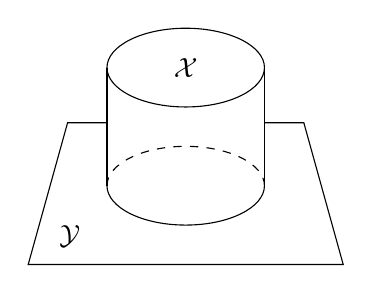
\begin{tikzpicture}[baseline=(O)]
	\draw (1, 1.5) ellipse[x radius=1, y radius=0.5] node {$\mathcal{X}$};
	\draw (0, 0) arc[start angle=180, end angle=360, x radius=1, y radius=0.5];
	\draw[dashed] (0, 0) arc[start angle=180, end angle=0, x radius=1, y radius=0.5];
	\draw (2, 1.5) -- (2, 0);
	\draw (0, 1.5) -- (0, 0);
	\draw (0, 0.8) -- (-0.5, 0.8) -- (-1, -1) node[xshift=1.5em,  yshift=1em] {$\mathcal{Y}$} -- (3, -1) -- (2.5, 0.8) -- (2, 0.8);
	\coordinate (O) at (0, 0.5);
\end{tikzpicture} \quad
	\Cone_{\mathrm{top}}(F) = 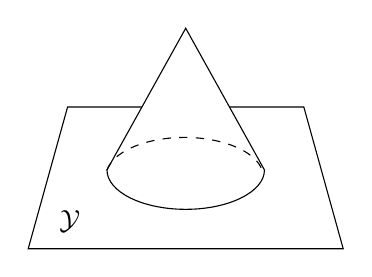
\begin{tikzpicture}[baseline=(O)]
	\draw (0, 0.8) -- (-0.5, 0.8) -- (-1, -1) node[xshift=1.5em,  yshift=1em] {$\mathcal{Y}$} -- (3, -1) -- (2.5, 0.8) --cycle;
	\filldraw[fill=white] (1, 1.8) -- (0, 0) arc[start angle=180, end angle=360, x radius=1, y radius=0.5] --cycle;
	\draw[dashed] (0, 0) arc[start angle=170, end angle=10, x radius=1, y radius=0.5];
	\coordinate (O) at (0, 0.5);
\end{tikzpicture}\]

% segment-id: o014.li2.chapter8.mapping-cone-revisited.p003
Himpunan simplisial memberikan cara konkret untuk menguraikan ruang
topologis. Secara lebih tepat, Teorema~\ref{prop:geom-Sing-adjunction}
memberikan pasangan adjoin
% segment-id: o014.li2.chapter8.mapping-cone-revisited.q004
\[\begin{tikzcd}
	{|\cdot|}: \cate{sSet} \arrow[shift left, r] & \cate{Top}: \mathrm{Sing}, \arrow[shift left, l]
\end{tikzcd}\]
dan kedua kategori tersebut memodelkan teori homotopi yang ekuivalen dalam
pengertian yang tepat. Konstruksi yang sama berlaku bila $\cate{Top}$ diganti
oleh $\cate{CGHaus}$. Sekarang kita terjemahkan pembahasan di atas ke
$\cate{sSet}$. Kita boleh mengandaikan
% segment-id: o014.li2.chapter8.mapping-cone-revisited.q005
\[ \mathcal{X} = |X|, \quad \mathcal{Y} = |Y|, \quad F = |f|: |X| \to |Y|, \]
dengan $f:X\to Y$ morfisme dalam $\cate{sSet}$. Dari sudut pandang
himpunan simplisial, kerucut pemetaan lebih mudah dijelaskan daripada
silinder pemetaan. Kita mulai dari kerucut $\mathcal{X}$,
$\Cone_{\mathrm{top}}(\mathcal{X}):=
\Cone_{\mathrm{top}}(\identity_{\mathcal{X}})$. Jika
$\mathcal{X}=|X|$, maka
$\Cone_{\mathrm{top}}(\mathcal{X})\simeq|X^{\lhd}|\simeq|X^{\rhd}|$
(Contoh~\ref{eg:cone-realization}). Di bawah ini kita berfokus pada
kerucut kiri $X^{\lhd}=\Delta^0\star X$ dan kompleks rantai yang
bersesuaian.
\index{himpunan simplisial!kerucut (cone)}

% segment-id: o014.li2.chapter8.mapping-cone-revisited.p004
Untuk setiap himpunan simplisial $Z$, tuliskan $Z_n^{\mathrm{nd}}$ untuk
himpunan semua simpleks-$n$ nondegenerat di dalamnya, dan tuliskan
$\{\mathrm{pt}\}=(\Delta^0)_0=(\Delta^0)_0^{\mathrm{nd}}$.
Proposisi~\ref{prop:join-nd}, atau intuisi topologis, memberikan
% segment-id: o014.li2.chapter8.mapping-cone-revisited.q006
\begin{equation}\label{eqn:Cone-X-aux1}
	(\Delta^0 \star X)^{\mathrm{nd}}_n = \begin{cases}
		X^{\mathrm{nd}}_n \sqcup \left( \{ \mathrm{pt} \} \times X^{\mathrm{nd}}_{n-1} \right), & n > 0 \\
		\{\mathrm{pt}\} \sqcup X_0, & n = 0.
	\end{cases}
\end{equation}

% segment-id: o014.li2.chapter8.mapping-cone-revisited.p005
Dengan mensubstitusikan \eqref{eqn:join-formulas} dan rumus umum yang
dibahas di atasnya, tampak bahwa untuk $n\geq1$, pembatasan
$d_i:(\Delta^0\star X)_n\to(\Delta^0\star X)_{n-1}$ pada
$\{\mathrm{pt}\}\times X_{n-1}$ dan $X_n$ adalah sebagai berikut:
% segment-id: o014.li2.chapter8.mapping-cone-revisited.q007
\begin{equation}\label{eqn:Cone-X-aux2}\begin{gathered}
	\begin{tikzcd}[column sep=small,
		/tikz/execute at end picture={
			\node [rectangle, draw, fit=(A) (B)] {};
			\node at ($(A)!.5!(C) + (0, 0.8)$) {$1 \leq i \leq n$};
		}]
		|[alias=A]| \{\mathrm{pt}\} \times X_{n-1} \arrow[d, "{\identity \times d_{i-1}}"'] & |[alias=C]| X_n \arrow[d, "{d_i}"] \\
		\{\mathrm{pt}\} \times X_{n-2} & |[alias=B]| X_{n-1}
	\end{tikzcd} \quad
	\begin{tikzcd}[column sep=small,
		/tikz/execute at end picture={
			\node [rectangle, draw, fit=(A) (B)] {};
			\node at ($(A)!.5!(C) + (0, 0.8)$) {$i=0$};
		}]
		|[alias=A]| \{\mathrm{pt}\} \times X_{n-1} \arrow[rd, "{\mathrm{pr}_2}"] & |[alias=C]| X_n \arrow[d, "{d_0}"] \\
		\{\mathrm{pt}\} \times X_{n-2} & |[alias=B]| X_{n-1}
	\end{tikzcd}
\end{gathered}\end{equation}
Jika $n=1$, $\{\mathrm{pt}\}\times X_{n-2}$ dalam rumus ini harus
dipahami sebagai $\{\mathrm{pt}\}$.

% segment-id: o014.li2.chapter8.mapping-cone-revisited.p006
Karena tujuan kita ialah kompleks rantai, langkah berikutnya adalah
melinearkan masalah melalui funktor $\Z(\mathord\cdot)$ dari
Definisi~\ref{def:free-simplicial-Ab}, lalu beralih ke kompleks rantai
melalui korespondensi Dold--Kan:
% segment-id: o014.li2.chapter8.mapping-cone-revisited.q008
\begin{equation*}
	\mathrm{N}(\Z X^{\lhd}) \simeq \mathrm{C}(\Z X^{\lhd}) \big/ \text{bagian degenerat} \quad \text{(Proposisi \ref{prop:Dold-Kan-v})}.
\end{equation*}
Untuk menyingkat notasi dalam sisa bagian ini, kita tulis
$\mathrm{N}X:=\mathrm{N}(\Z X)$ dan
$\mathrm{N}f:=\mathrm{N}(\Z f)$. Struktur kompleks rantai
$\mathrm{C}(\Z X^{\lhd})$ berasal dari
$\partial_n:=\sum_{i=0}^n(-1)^id_i$. Dengan menggabungkan
\eqref{eqn:Cone-X-aux1}, \eqref{eqn:Cone-X-aux2}, dan deskripsi
$\Cone(\identity_{\mathrm{N}X})$ dalam Catatan~\ref{rem:cone-chain},
diperoleh barisan eksak pendek kompleks rantai
% segment-id: o014.li2.chapter8.mapping-cone-revisited.q009
\[ 0 \to \underbracket{\Z\{\mathrm{pt}\}}_{\text{derajat nol}} \to \mathrm{N}(\Z X^{\lhd}) \to \Cone(\identity_{\mathrm{N}X}) \to 0. \]

% segment-id: o014.li2.chapter8.mapping-cone-revisited.p007
Selanjutnya, funktor $|\mathord\cdot|$ dan
$\mathrm{N}\Z(\mathord\cdot)$ mempertahankan diagram dorongan keluar:
yang pertama merupakan funktor adjoin kiri, sedangkan yang kedua merupakan
komposisi funktor adjoin kiri dengan suatu ekuivalensi; dalam topologi, diagram dorongan keluar
berarti perekatan. Karena itu, untuk $f:X\to Y$ definisikan
% segment-id: o014.li2.chapter8.mapping-cone-revisited.q010
\begin{equation*}
	\Cone_{\mathrm{s}}(f) := X^{\lhd} \dsqcup{X, f} Y.
\end{equation*}
Kemudian kita memperoleh
% segment-id: o014.li2.chapter8.mapping-cone-revisited.q011
\[\begin{tikzcd}
	\mathcal{X} \arrow[d, "F"'] \arrow[r, "{\text{dasar}}"] & \Cone_{\mathrm{top}}(\mathcal{X}) \arrow[d] \\
	\mathcal{Y} \arrow[r] & \Cone_{\mathrm{top}}(F) \arrow[phantom, lu, "\boxplus" description]
\end{tikzcd} \xleftarrow{|\cdot|} \begin{tikzcd}
	X \arrow[d, "f"'] \arrow[r, "\text{kanonik}"] & X^{\lhd} \arrow[d] \\
	Y \arrow[r] & \Cone_{\mathrm{s}}(f) \arrow[phantom, lu, "\boxplus" description]
\end{tikzcd} \xrightarrow{\mathrm{N}} \begin{tikzcd}
	\mathrm{N}X \arrow[d, "{\mathrm{N}f}"'] \arrow[r] & \mathrm{N}X^{\lhd} \arrow[d] \\
	\mathrm{N}Y \arrow[r] & \mathrm{N}\Cone_{\mathrm{s}}(f) \arrow[phantom, lu, "\boxplus" description]
\end{tikzcd}\]
Rangkaian konstruksi ini menunjukkan bahwa padanan aljabar linear dari
$\Cone_{\mathrm{top}}(F)$ seharusnya ialah
$\mathrm{N}\Cone_{\mathrm{s}}(f)$.

% segment-id: o014.li2.chapter8.mapping-cone-revisited.pr001
\begin{proposition}\label{prop:Cone-comparison}
	\index{kerucut pemetaan@kerucut pemetaan}
	Dengan notasi di atas, terdapat barisan eksak pendek kanonik kompleks
	rantai
	% segment-id: o014.li2.chapter8.mapping-cone-revisited.q012
	\[ 0 \to \underbracket{\Z\{\mathrm{pt}\}}_{\text{derajat nol}} \to \mathrm{N}\Cone_{\mathrm{s}}(f) \to \Cone(\mathrm{N}f) \to 0. \]
\end{proposition}
\begin{proof}
	Dorongan keluar tidak memengaruhi subkompleks rantai
	$\Z\{\mathrm{pt}\}$ dari $\mathrm{N}X^{\lhd}$, yang bersesuaian
	dengan puncak kerucut. Pada derajat $n$, ia mengganti semua $X_n$ dengan
	$Y_n$ dan mengganti proyeksi $\mathrm{pr}_2$ dalam
	\eqref{eqn:Cone-X-aux2} dengan $f_{n-1}\mathrm{pr}_2$. Karena itu, pada
	tingkat hasil bagi $\Cone(\identity_{\mathrm{N}X})$, hasil dorongan
	keluar tersebut adalah tepat $\Cone(\mathrm{N}f)$; lihat
	Catatan~\ref{rem:cone-chain}.
\end{proof}

% segment-id: o014.li2.chapter8.mapping-cone-revisited.r001
\begin{remark}
	Silinder pemetaan $\Cyl_{\mathrm{top}}(F)$ dan versi kompleks rantainya
	dapat dibandingkan dengan cara serupa; dalam hal ini tidak perlu lagi
	mengambil hasil bagi oleh sumbangan puncak. Akan tetapi, silinder
	pemetaan melibatkan hasil kali himpunan simplisial, sedangkan
	$\mathrm{N}$ bukan funktor monoidal. Karena itu, penjelasan topologis
	biasanya menggunakan kompleks CW, bukan himpunan simplisial, sebab hasil
	kali lebih mudah ditangani dalam dunia kompleks CW.
\end{remark}

% segment-id: o014.li2.chapter8.mapping-cone-revisited.p008
Singkatnya, kerucut pemetaan kompleks rantai adalah hasil bagi kerucut
pemetaan yang berasal dari himpunan simplisial (atau topologi) oleh satu
salinan $\Z$ yang berasal dari puncak $\mathrm{pt}$. Dalam studi kompleks
rantai, peran utama kerucut pemetaan ialah bahwa setiap pemetaan
$\phi:A\to B$ meluas menjadi barisan
% segment-id: o014.li2.chapter8.mapping-cone-revisited.q013
\begin{equation}\label{eqn:cofiber-comparison-A}
	A \xrightarrow{\phi} B \to \Cone(\phi) \to A[-1] \xrightarrow{-\phi[-1]} B[-1] \to \cdots .
\end{equation}

% segment-id: o014.li2.chapter8.mapping-cone-revisited.p009
Dalam situasi topologis, pemetaan yang bersesuaian dengan
$\Cone(\phi)\to A[-1]$ diperoleh dengan mengerutkan dasar
$\mathcal{Y}$ dari $\Cone_{\mathrm{top}}(F)$ menjadi satu titik. Hasil
pengerutan itu dinotasikan oleh $S\mathcal{X}$; ia tidak bergantung pada
$\mathcal{Y}$ (lihat gambar di bawah) dan memberikan sebuah funktor $S$.
Barisan pemetaan yang bersesuaian ialah
% segment-id: o014.li2.chapter8.mapping-cone-revisited.q014
\begin{equation*}
	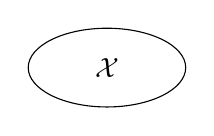
\begin{tikzpicture}[baseline=(O)]
		\draw (1, 0) ellipse[x radius=1, y radius=0.5] node {$\mathcal{X}$};
		\coordinate (O) at (0, 0);
	\end{tikzpicture}
	\xrightarrow{F}
	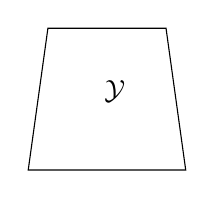
\begin{tikzpicture}[baseline=(O), xscale=0.5]
		\draw (0, 0.8) -- (-0.5, 0.8) -- (-1, -1) -- (3, -1) -- (2.5, 0.8) --cycle;
		\node at (1.2, 0) {$\mathcal{Y}$};
		\coordinate (O) at (0, 0.5);
	\end{tikzpicture}
	\xrightarrow{\text{inklusi}}
	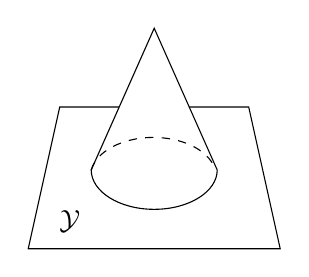
\begin{tikzpicture}[baseline=(O), xscale=0.8]
		\draw (0, 0.8) -- (-0.5, 0.8) -- (-1, -1) node[xshift=1.5em,  yshift=1em] {$\mathcal{Y}$} -- (3, -1) -- (2.5, 0.8) --cycle;
		\filldraw[fill=white] (1, 1.8) -- (0, 0) arc[start angle=180, end angle=360, x radius=1, y radius=0.5] --cycle;
		\draw[dashed] (0, 0) arc[start angle=170, end angle=10, x radius=1, y radius=0.5];
		\coordinate (O) at (0, 0.5);
	\end{tikzpicture}
	\xrightarrow{\text{kerut}}
	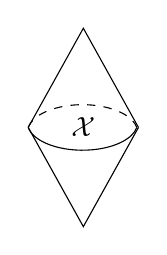
\begin{tikzpicture}[baseline=(O), xscale=0.7, yscale=0.7]
		\draw (2, 0) -- (1, 1.8) -- (0, 0);
		\draw[dashed] (0, 0) arc[start angle=170, end angle=10, x radius=1, y radius=0.5];
		\draw (0, 0) arc[start angle=190, end angle=350, x radius=1, y radius=0.5];
		\node at (1, 0) {$\mathcal{X}$};
		\draw (0, 0) -- (1, -1.8) -- (2, 0);
		\coordinate (O) at (0, 0.5);
	\end{tikzpicture}
	\to \cdots .
\end{equation*}
Barisan ini disebut \emph{barisan kofiber} yang dihasilkan oleh $f$
(lebih tepatnya, versi tanpa titik pangkal). Jika kita bekerja dalam
$\cate{sSet}$ dan mengambil kompleks rantai dari barisan yang bersesuaian,
hasilnya kira-kira \eqref{eqn:cofiber-comparison-A}. Kata ``kira-kira''
diperlukan karena:
\begin{itemize}
	\item Pemetaan $S\mathcal{X}\to S\mathcal{Y}$ tidak dapat sekadar
	didefinisikan sebagai $S(F)$; koordinat vertikal harus dibalik dengan tepat.
	Pada tingkat aljabar linear, hal ini bersesuaian dengan
	$-\phi[-1]$ dalam \eqref{eqn:cofiber-comparison-A}; lihat buku ajar
	topologi untuk perinciannya.
	\item Seperti terlihat dalam Proposisi~\ref{prop:Cone-comparison},
	berbagai kompleks rantai mengandung satu salinan $\Z$ berlebih yang
	bersesuaian dengan puncak ruang-ruang seperti
	$\Cone_{\mathrm{top}}(F)$ dan $S\mathcal{X}$. Dalam topologi, persoalan
	ini dihindari dengan memakai ruang bertitik pangkal, lalu dalam
	konstruksi topologis kerucut mengerutkan bagian yang terhubung dengan
	titik pangkal tersebut.
\end{itemize}

% segment-id: o014.li2.chapter8.mapping-cone-revisited.p010
Jika untuk sementara semua perincian dikesampingkan, secara garis besar
teori kategori turunan yang dibangun dalam \S\ref{sec:derived-cat}, dengan
$\mathcal{A}=\cate{Ab}$, dapat pula dipandang sebagai ``linearisasi'' yang
agak kasar dari teori homotopi\footnote{Lebih tepatnya teori homotopi
stabil, karena kompleks rantai membolehkan suku berderajat negatif.}.

% segment-id: o014.li2.chapter8.mapping-cone-revisited.p011
Karena persoalan-persoalan terkait semakin melibatkan gagasan dan metode
topologis, kita berhenti di sini agar tidak menyimpang terlalu jauh.
